\chapter{Background\label{cha:background}}

In this chapter, we discuss traditional artificial intelligence in the context of search, and explain the algorithms we used. Additionally, we discuss similar methods for searching state-spaces. We allocate a large portion of the section to Breakthrough as that will be our testbed. We discuss the different classes of machine learning as well as neural networks.

\section{Environments}
\label{sec:environments}

When researching artificial intelligence it is important to select an environment that is a suitable abstraction for the task at hand. Environments vary significantly and can be identified by their characteristics. The characteristics that are commonly used to describe environments can be seen in Table~\ref{tab:env_characteristics}\cite{Russell:AIModern}.

\begin{table}[ht]
	\centering
	\caption{Characteristics of environments}
	\begin{tabular}{|c|c|p{6cm}|}
		\hline
		\textbf{characteristic} & \textbf{Values}              & \textbf{Description}                                                                 \\
		\hline
		Observable              & Fully, Partially             & How much of the environment can your agent percieve.                                 \\
		\hline
		Agents                  & Single, Multi                & Are there multiple agents playing in the environment.                                \\
		\hline
		Deterministic           & Deterministic, Stochastic    & Do the actions your agents execute deterministicly impact the environment.                 \\
		\hline
		Episodic                & Sequential, Episodic         & Are actions episodic or sequential.                                                  \\
		\hline
		Static                  & Static, Semi-Static, Dynamic & Does the environment change without agent input, or does it wait until agents take actions. \\
		\hline
		Discrete                & Discrete, Continuous         & Is your environment discrete w.r.t actions.                                          \\
		\hline
	\end{tabular}
	\label{tab:env_characteristics}
\end{table}

Categorizing environments using Table \ref{tab:env_characteristics} gives one the power to find an environment in which a method works and know it can be applied to different environments with the same characteristics. Additionally, it allowes us to talk about agents in the context of environments as the entities that act within the environment.

\section{Game Environment}

Classical artificial intelligence game environments are commonly used to validate a method, e.g game environments can be games like Tic-Tac-Toe or Breakthrough, or simluation environments like driving simulators. Game environments are a suitable place to apply AI as they serve as an abstraction of the real world, for instance, a self-driving car agent who is verified to avoid driving into walls in a simulation is possibly safer than one who is not.

\section{Breakthrough}

The game Breakthrough is a simplified version of chess; the game is set up on a $M\times N$ board with squares like in chess, and each player starts with two rows of pawns at opposite ends. The objective of the game is for a player to move one of their pawns to the opposite end of the board. A player wins if either they have reached the opposite end of the board or have captured all of his opponents' pawns. The pawns differ from chess pawns in such a way that they can not move two squares on the first move and they can both move and capture diagonally. This leads to the game being impossible to draw as pieces are always able to move or capture. An example of an initial board in Breakthrough can be seen in Figure~\ref{fig:initbtboard}. 

\begin{figure}[]
	\centering

	\breakthrough{8/8/pppppp2/pppppp2/8/8/PPPPPP2/PPPPPP2 w - - 0 1}

	\caption{Initial Breakthrough board}
	\label{fig:initbtboard}
\end{figure}


\begin{table}[ht]
	\centering
	\caption{Categorization of Breakthrough}
	\begin{tabular}{|c|c|}\hline
		\textbf{Characteristic} & \textbf{Value} \\\hline
		Observable              & Fully          \\\hline
		Agents                  & Multi          \\\hline
		Deterministic           & Deterministic  \\\hline
		Episodic                & Sequential     \\\hline
		Static                  & Static         \\\hline
		Discrete                & Discrete       \\\hline
	\end{tabular}
	\label{tab:breakthrough_cat}
\end{table}

Categorizing Breakthrough with the characteristics described in Section~\ref{sec:environments} we end up with the description shown in Table~\ref{tab:breakthrough_cat}. These characteristics are identical to that of Tic-Tac-Toe, and chess. This categorization is the most common in board games where two players compete.

\subsection{Heuristics of Breakthrough}

To evaluate the game of Breakthrough we may consider many heuristics (higher-level concepts), for instance a very simple heuristic would be a players material advantage. \textit{Material Advantage} is the amount of pieces the player has minus the amount of pieces the opponent has. This heuristics gives us some insight into how well the game is progressing, but obviously, there are cases where this does not tell us much, for example when your opponent has a single piece left that is on the row immediately before the row needed for them to win. No matter how many pieces you have left, this state is bad for you if you're not able to capture that piece. An example of such a state can be seen in Figure~\ref{fig:bt_h1_bad}.

\begin{figure}[]
	\centering
	\breakthrough{8/8/pppp4/pp3P2/2p5/8/8/8 w - - 0 1}
	\caption{Breakthrough board where Material Advantage doesn't work well}
	\label{fig:bt_h1_bad}
\end{figure}

A different heuristic would be the distance of your most advanced pawn minus your opponent's most advanced pawn; this could give you insight into how close you are to winning the game or how close your opponent is. As a higher-level concept, we can call this concept your \textit{aggressiveness}, as it closely resembles how aggressive you are going for the win. Generally, in Breakthrough, it is favorable to move your whole team as a unit and play more defensively\cite{lorentz:heuristic}. More advanced heuristics for Breakthrough will be discussed in detail later in a later chapter.

\section{State-Space Search}

Traditionally, methods for playing games search through the environment using a heuristic to guide the search. A simple way of doing a heuristic-based search would be to give all non-terminal states a $0$ score and terminal states positive or negative scores based on whether it is a win or a loss, repesctively. We say that that a search algorithm is not guided, and the algorithm will probably have to evaluate a large portion of the state-space. This method of searching is generally extremely inefficient as the state-spaces of game environments are often extremely large, even infinite. For instance, an upper-bound estimate of the state-space for Breakthrough is $3^{(M-1)*(N-1)}+2*N$ where $M$ is the height of the board $N$ is the width of the board. The $3^{(M-1)*(N-1)}$ represents each position of the board having either a white, or black piece, or being empty. And, the $2*N$ component represents each square the final piece to move could have moved to. So for a small board, $5\times 4$ the upper-bound estimation of the state-space is $531{,}449$ states.

This is why a good heuristic is needed because we can identify paths in the game tree that will lead to a bad outcome early, allowing us to disregard a significant amount of states, reducing the time required to search.

The algorithms that are used in traditional state-space search are for instance Depth-first search (DFS), Breadth-first Search (BFS), Alpha-Beta Search (AB-Search)\cite{abpruning:dj}, and Monte-Carlo Tree Search (MCTS).

More modernly, these search methods have been augmented by Machine Learning, in such a way that we do not need to figure out a good heuristic for a given state, but rather, we apply a machine learning model to learn a function that takes in a state and returns an evaluation of that state\cite{neuralnetworksgames:michulke}. This can lead to a significant time reduction as we do not need to simulate a whole game from a state to receive its evaluation but rather receive the evaluation from the model.

\subsection{Monte-Carlo Tree Search}

\label{sec:mcts}

In the algorithm Monte-Carlo Tree Search, described by R. Coulom\cite{mcts:coulom}, there is an agent within an environment. Each node in the environment represents a state of the environment, and each edge from the node represents a possible action from that state $s$ to a child state $s'$. Often, these concepts are considered state-action pairs, which should be unique within the environment. And as such, they create a tree where we are able to search the state-space.

MCTS is a method of exploring an environment in a best-first manner. In MCTS there are four stages: Selection, Expansion, Simulation, and Back-propagation. They happen sequentially and repeatedly. MCTS is initialized with a tree consisting of the unexpanded initial state of the environment. This tree consists of nodes $n_i$ where $i$ represents the point in time of game state, for example, $n_0$ in chess is the initial position and $n_x$ is some position in the middle of the game and $n_e$ is one of the states representing a position where there is either a draw or one player has won the match. Each of the nodes has $4$ values, $s$, $a$, $Q$, and $N$. These values represent these items, $s$ is the state of the environment, $a$ is the action that brought the previous node $n_{i-1}$ to node $n_i$, $Q$ is the average reward from running the MCTS algorithm from this node, and $N$ the number of times the MCTS algorithm has visited this node. The values $s$ and $a$ uniquely identify a position in the environment and are often called state-action pairs.

We describe the MCTS algorithm's four phases: Selection, Expansion, Simulation/Rollout, Backpropagation, in more detail below.

\begin{equation} \label{UCT_formula}
	\text{Child UCT value} = Q_{(s',a')} + c_{uct} * \frac{\sqrt{log(N_{(s,a)})}}{N_{(s',a')}}
\end{equation}

\subsection*{Selection}
During the selection phase, a node $s$ within the tree which has not yet been expanded is found.
This process uses Upper Confidence Bound on Trees (UCT)\cite{kocsis:uct} to find that node $s$, the formula is described in Equation \ref{UCT_formula}. For a parent node $s_{parent}$
(initially the root of the tree) we select the child with the highest UCT value repeatedly until an unexpanded
node is found. This process is done to balance the amount of exploration vs exploitation of nodes in the
tree.

\subsection*{Expansion}
Then the expansion phase expands the node generating all $s'$ nodes, the nodes are generated by applying all actions $a$ in $s$.

\subsection*{Rollout}
Next during rollout, actions $a$ from $s$ are randomly selected to move to $s'$, then repeated to go to $s''$, until a terminal node within the environment is reached. By terminal, we mean a state in which the game is finished. A terminal node in MCTS can generally return any value, but in the context of this paper, we only return (+1 white wins, or -1 black wins).


\subsection*{Backpropagation}
The result from the terminal node is then propagated up through the path taken by selection $(s,a)$ up
to the root of the tree, updating the $Q_{(s,a)}$ values of each node $(s,a)$.

\subsection{Neural Network based UCT}

When training a neural network the UCT formula is modified slightly to prefer selecting nodes
that the neural network values highly by introducing a second scalar to the formula $f((s,a)) = (p,v)$, where $f$ is the neural network, $p$ is the policy vector returned by the neural network and $v$ is the predicted value from the neural network. The resulting formula is described in Equation \ref{PUCT_formula}, and is called PUCT\cite{rosin:puct}. Secondly, the backpropagation process is modified to instead of doing rollout/simulation to receive a reward the predicted value $v$ from the neural network is used.

\begin{equation} \label{PUCT_formula}
	\text{Child PUCT value} = Q(s,a) + c_{puct} * p(s,a) * \frac{\sqrt{\sum_b{N(s,b)}}}{1+N(s,a)}
\end{equation}

\section{Machine Learning}

Machine Learning (ML) is a research field in which machines apply statistical functions on data to achieve a correct output, where by \textit{correct} we mean the corresponding result that we expect. Generally, this a repetitive process where we look at examples of the data, and the algorithm progressively gets closer to the underlying function of the data it is fed. This process is therefore similar to trial and error for humans. ML is a sub-field of Artificial Intelligence.

We can categorize machine learning into three different sub-categories: Supervised Learning, Reinforcement Learning, and Unsupervised Learning.

\subsection{Supervised Learning}

In Supervised Learning, the ML algorithms attempt to build a model from a data set of labelled examples. The labelled examples are a set of input values and their corresponding output value. The ML algorithm then uses this data set to construct a model that is as accurate as possible at outputting the correct output value given the input value. In supervised learning many techniques are applied to maintain the generality of the model s.t. it does not just represent the data set it is given but also has high accuracy on a possible future data set it has not yet encountered.

Some examples of algorithms that are popular for Supervised learning would be, Decision Trees, Support Vector Machines, or Naive Bayes.

\subsection{Reinforcement Learning}

Reinforcement Learning focuses on the idea of trial and error for an ML algorithm, where the algorithm directly interacts with the environment it operates in, and from operating in the environment it is provided with either positive or negative feedback for its actions. Typically, the environment needs to be modeled as a Markov Decision Process. That is, the selection of actions in a state requires only the knowledge of being in that state, not the actions it took to get to that state.

Many algorithms are popular in reinforcement learning, for instance Q-learning\cite{qlearning:watkins}, and TD-Lambda\cite{sutton:tdlambda}.

\subsection{Unsupervised Learning}

In Unsupervised Learning, the machine learning algorithms attempt to build a model from a data set of values that do not have a corresponding output value. These algorithms then generally attempt to find pattern within the data set, to which we could then later label upon examination of the patterns. Importantly, in Unsupervised Learning, all columns of values in the data set should be normalized to the same range, and should be standardized s.t. the mean of the values is $0$ and it's standard deviation is $1$. This is done in order for one value not to dominate the patterns in the data set.

Common algorithms in Unsupervised Learning are, K-Nearest Neighbours (KNN), K-Means\cite{lloyd:kmeans}, and DBScan\cite{ling:dbscan}.

\subsection{Neural Networks}

Neural networks (NN) are popular methods within a sub-field of ML known as Deep Learning (DL). Neural networks are generally used on a labelled dataset. NN's are created to resemble how the human brain functions. In the brain, we have neurons which when they receive a signal they apply some function to them and if the resulting signal is high enough, they fire to the next neuron. This is how it is done in the neural network model as well. In NNs we have a layer of neurons $f_i$, initial layer being $f_0$ and the last layer being $f_n$. These layers behave in such a way that when they get some input, generally a vector of numbers, each neuron in the layer takes the sum of that vector, weighs the sum by a learned weighing factor, then applies an activation function to it. The result of doing this is then passed on to the next neuron. Until a final layer of neurons is reached. At that point, we have reached a layer that corresponds to the prediction of the network. This value can be a binary classification (cat or dog image), a regression value (the value of a property), or even the neural networks representation of the input, e.g where a neural network attempts to create an image from an example image\cite{karras:stylegan}. It can then be said that a neural network is doing a function approximation of the input to some value. And, would be mathematically stated as $f_n ( w_n * f_{n-1} (w_{n-1} * \dots f_0(w_0*i))) = o$.

The core of the learning in neural networks comes from optimizing the weighing factor. That weighting factor is gradually made to move in the direction of the actual correct output by algorithms, e.g the backpropagation algorithm\cite{rumelhard:backprop}.


%\section{Traditional Learning in Board Games}

\section{Explainable Artificial Intelligence (XAI)}

The field of XAI research is still far behind its counterpart AI research\cite{tjoa:surveyxai}. Within XAI two fields are the largest: Model Interpretability and Model Explainability.

\subsection{Model Interpretability}

Model Interpretability is the more common approach of XAI, mainly because it is less constrained than model explainability. In order to achieve model interpretability, we must be able to answer the question of what prediction the model will return on a given input, with a high accuracy. Simple examples would be, given a trained neural network and a picture of a dog, if that model is highly interpretable, we can say with high certainty that the predicted value will be dog.

\subsection{Model Explainability}

Model explainability within the context of neural networks is not possible today. Model
explainability refers to firstly considering some input and output from a model. Then
afterwards the model is examined to determine exactly what led to the predicted output.
This concept is simple when we're working with Decision Trees. A decision tree is a tree
whose nodes are representative of an input value and at every node a branch is selected
based on the value of the input value. It is therefore easy to see how to examine the tree
to explain the output. By following the branches in the tree we can exactly explain why the model predicted the output.

When we talk about neural networks this process is much more difficult; the underlying nodes
are generally in the millions and the different layers of the neural network vary in the operations they apply to the input. During this process, the value is modified such that it becomes far removed from the initial input value. That being said, while the possibility of completely monitoring the training process and completely monitoring the evaluation process is possible it is not feasible.


\subsection{Saliency Maps}

Within XAI many methods have been developed to try to explain
ANN's. In the field of image recognition there has been a lot of work examining which
pixels of an image the model deems important. One such method is Saliency Maps\cite{Koch:saliency}. There the pixel values the model
deems important are colored s.t. a human can examine the image and get a
sense of what portions of the image are important to the model. An example of
a classification of a dog can be seen in Figure \ref{fig:dog_saliency}. This method is understandable to a human when the saliency map lines up to what we would focus on. However, this achieves no explanation on the prediction if the saliency map doesn't line up to human intuition or the prediction, for example, if in the same Figure \ref{fig:dog_saliency} we had the same saliency map but the prediction would be dragon, or if the salience map was on the trees and the prediction was dog.

\begin{figure}[]
	\centering
	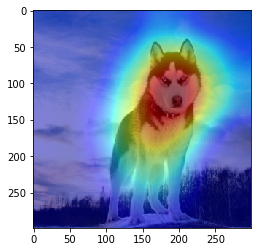
\includegraphics[width=.5\textwidth]{graphics/dog_saliency}
	\caption{Example of a model's saliency map for an image of a dog}
	\label{fig:dog_saliency}
\end{figure}

\subsection{Shapley Values}

Methods for explaining models that are not image recognition models include
Shapley values, from Lundberg \& Lee\cite{LundbergL:shapley}. There the input is examined against its output, then iteratively
input values are selected to be fixed. Then the other input values are varied and
an average change in prediction is calculated. With this the Shapley value can be
estimated for the fixed input value. This is done to examine which input values have
the strongest link to the output value. Shapley values on a dataset can give insights
on which input values the model deems most important.

\subsection{Concept Activation Vectors}

A recent paper by Been Kim et al.\cite{Keem:TCAV}, shows a method for examining
a neural network giving a much more humanlike insight into a prediction. Using Concept
Activation Vectors (CAV) a directional derivative for a given input can be examined
with respect to some HLC's. For example, when a human looks at an image of an animal
and is supposed to decide whether the image is of a horse or a zebra, an intuitive
approach would be to check whether the animal has stipes, or the animal has both white and black colors.
That method of determining if a horse is a zebra could then be called a higher-level
concept, and if we're able to gather if a nerual network uses this strategy for prediction
we have a deeper understanding of its underlying structure, leading to an explanation of
the result.

The construction of a CAV requires a method of labelling the values in your dataset with
the corresponding concept in order to create a binary classifier on data. The binary classifier is constructed on the internal representation of the data points within the neural network. After training the neural network, and constructing the classifier, we run a new datapoint through the neural network and we examine the directional derivative of that datapoint. If the direction is in the direction of the binary classifier we say that the datapoint contains the concept.

\section{Summary}

This section discussed some of the important algorithms related to the research done in this thesis, as well as giving a foundation in the readers understanding of the test bed we will be using in future sections.